\documentclass[tikz]{standalone}

\begin{document}
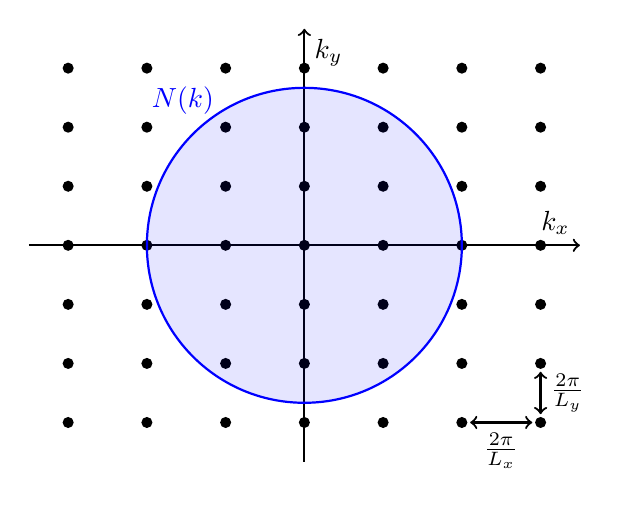
\begin{tikzpicture}[thick]

  % Dot grid
  \def\xrange{3}
  \def\yrange{3}
  \def\ratio{3/4}
  \foreach \x in {-\xrange,...,\xrange}
    {\foreach \y in {-\yrange,...,\yrange}
        {\fill (\x,\ratio*\y) circle[radius=2pt];}}

  % Axes
  \draw[->] (-\xrange-1/2,0) -- (\xrange+1/2,0) node[above left] {$k_x$};
  \draw[->] (0,-\ratio*\yrange-1/2) -- (0,\ratio*\yrange+1/2) node[below right] {$k_y$};

  % Lattice spacing
  \draw[<->,shorten >=3,shorten <=3] (\xrange-1,-\ratio*\yrange) -- (\xrange,-\ratio*\yrange) node[midway,below] {$\frac{2 \pi}{L_x}$};
  \draw[<->,shorten >=3,shorten <=3] (\xrange,-\ratio*\yrange) -- (\xrange,-\ratio*\yrange+\ratio) node[midway,right] {$\frac{2 \pi}{L_y}$};

  % Circle
  \draw[blue,fill=blue,fill opacity=0.1] (0,0) circle (2/3*\yrange);
  \node[blue] at (130:2.4) {$N(k)$};
\end{tikzpicture}
\end{document}
